\section{Metodologi \& Dataset}

\begin{frame}{Dataset \& Preprocessing}
    \begin{columns}
        \begin{column}{0.5\textwidth}
            \textbf{Deskripsi Data:}
            \begin{itemize}
                \item \textbf{Sumber:} LibriVox Indonesia (Terjemahan Deklarasi HAM / UDHR ke Bahasa Minangkabau).
                \item \textbf{Kuantitas:} 156 file audio dengan total durasi $\sim$1,3 jam.
                \item \textbf{Text Preprocessing:}
                \begin{itemize}
                    \item Case folding (huruf kecil).
                    \item Pembersihan tanda baca khusus (\textit{punctuation removal}).
                    \item Pembuangan karakter non-alfabet.
                \end{itemize}
            \end{itemize}
        \end{column}
        \begin{column}{0.5\textwidth}
            \textbf{Skema Validasi \& Eksperimen:}
            \begin{itemize}
                \item Menggunakan \textbf{5-Fold Cross-Validation}.
                \item Bertujuan mengoptimalkan set data yang sangat terbatas dan memastikan tidak ada bias dari \textit{random seed} tertentu.
                \item Pada setiap iterasi 5 fold: 4 fold untuk \textit{training}, 1 fold untuk \textit{evaluation}.
                \item Augmentasi hanya diterapkan pada data \textit{training} untuk menjaga integritas evaluasi. 
            \end{itemize}
        \end{column}
    \end{columns}
\end{frame}

\begin{frame}{Arsitektur Dasar: OpenAI Whisper}
    \begin{columns}
        \begin{column}{0.5\textwidth}
            \begin{figure}
                \centering
                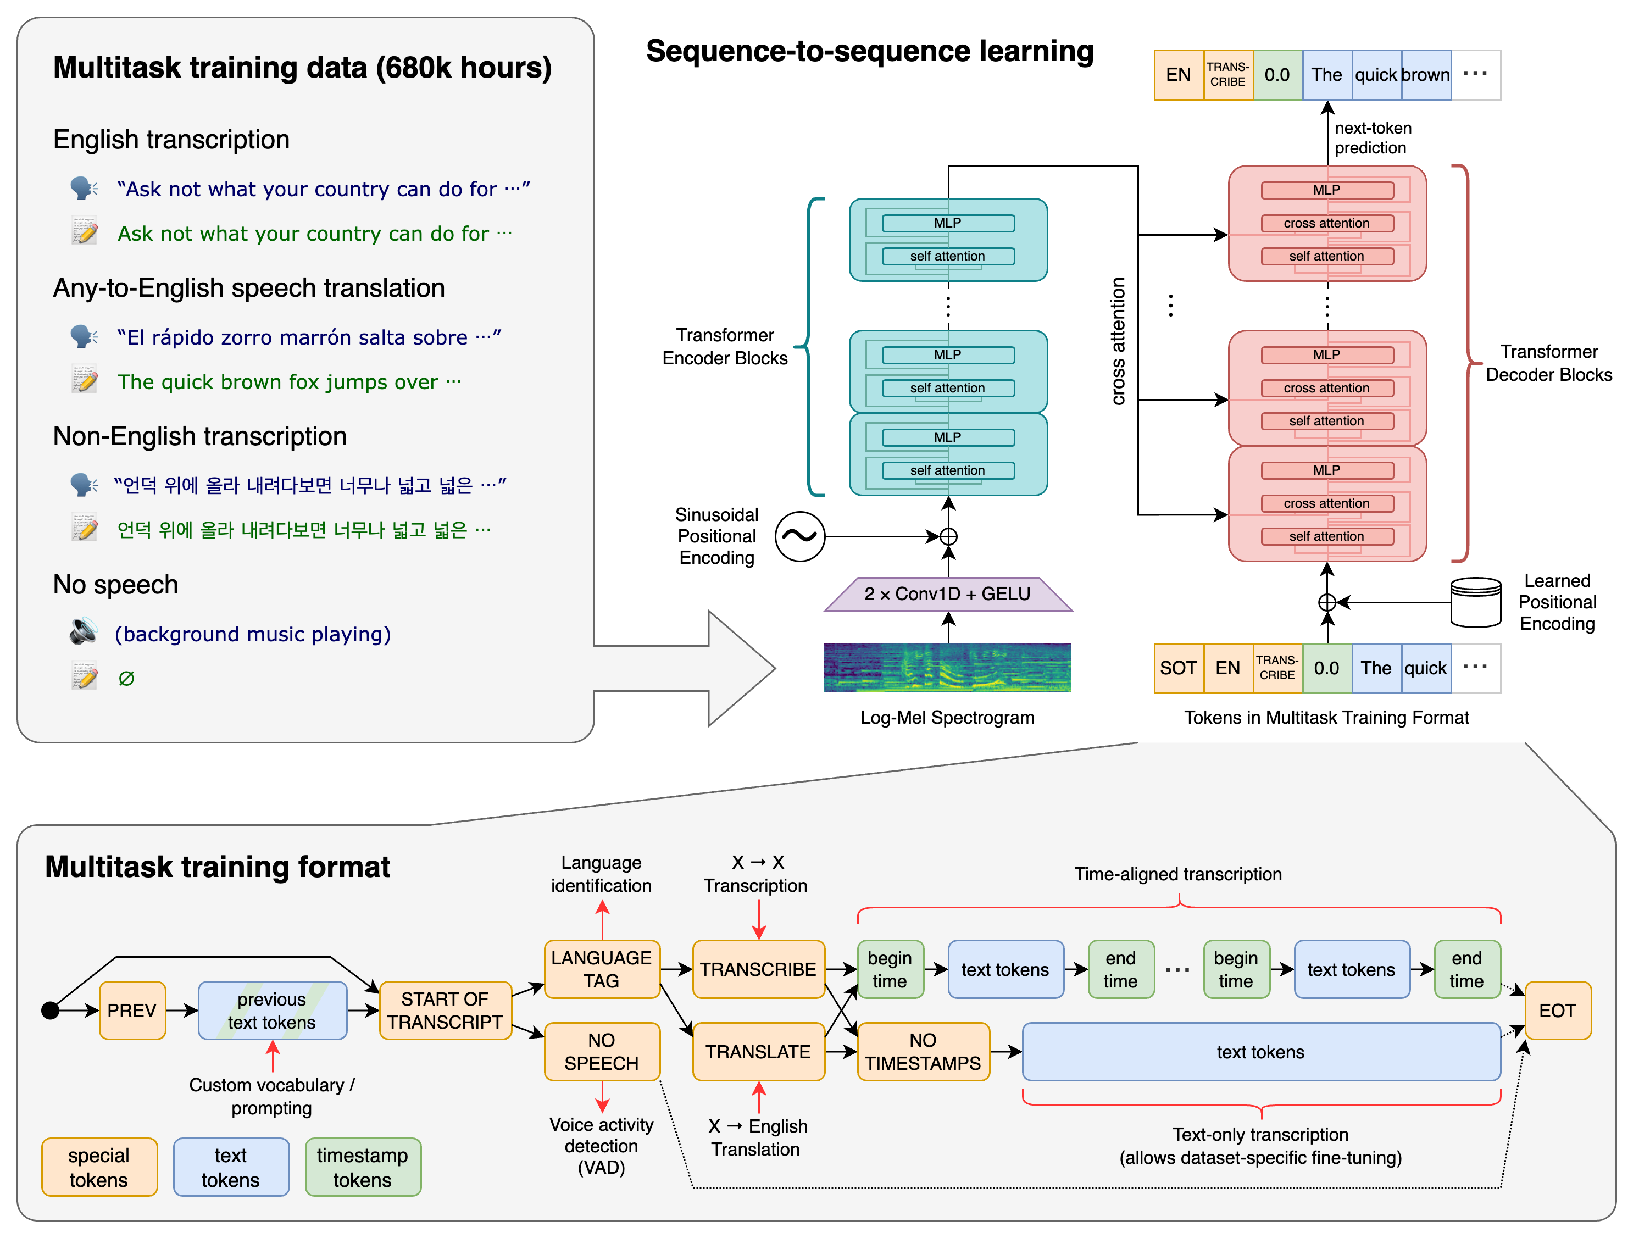
\includegraphics[width=\textwidth]{../figure/Whisper_Architecture.pdf}
                \caption{Arsitektur OpenAI Whisper}
            \end{figure}
        \end{column}
        \begin{column}{0.5\textwidth}
            \textbf{Whisper Base Model}
            \begin{itemize}
                \item \textbf{Total Parameter:} 74 juta.
                \item Arsitektur \textbf{Encoder-Decoder Transformer}.
                \item Memproyeksikan fitur audio (\textit{Log-Mel Spectrogram}) menjadi barisan token bahasa melalui atensi (\textit{cross-attention}).
                \item Sudah \textit{pre-trained} multibahasa, namun tetap perlu adaptasi untuk bahasa \textit{extremely low-resource} seperti Minangkabau.
            \end{itemize}
        \end{column}
    \end{columns}
\end{frame}

\begin{frame}{Alur Penelitian \& Validasi}
    \begin{columns}
        \begin{column}{0.56\textwidth}
            \begin{figure}
                \centering
                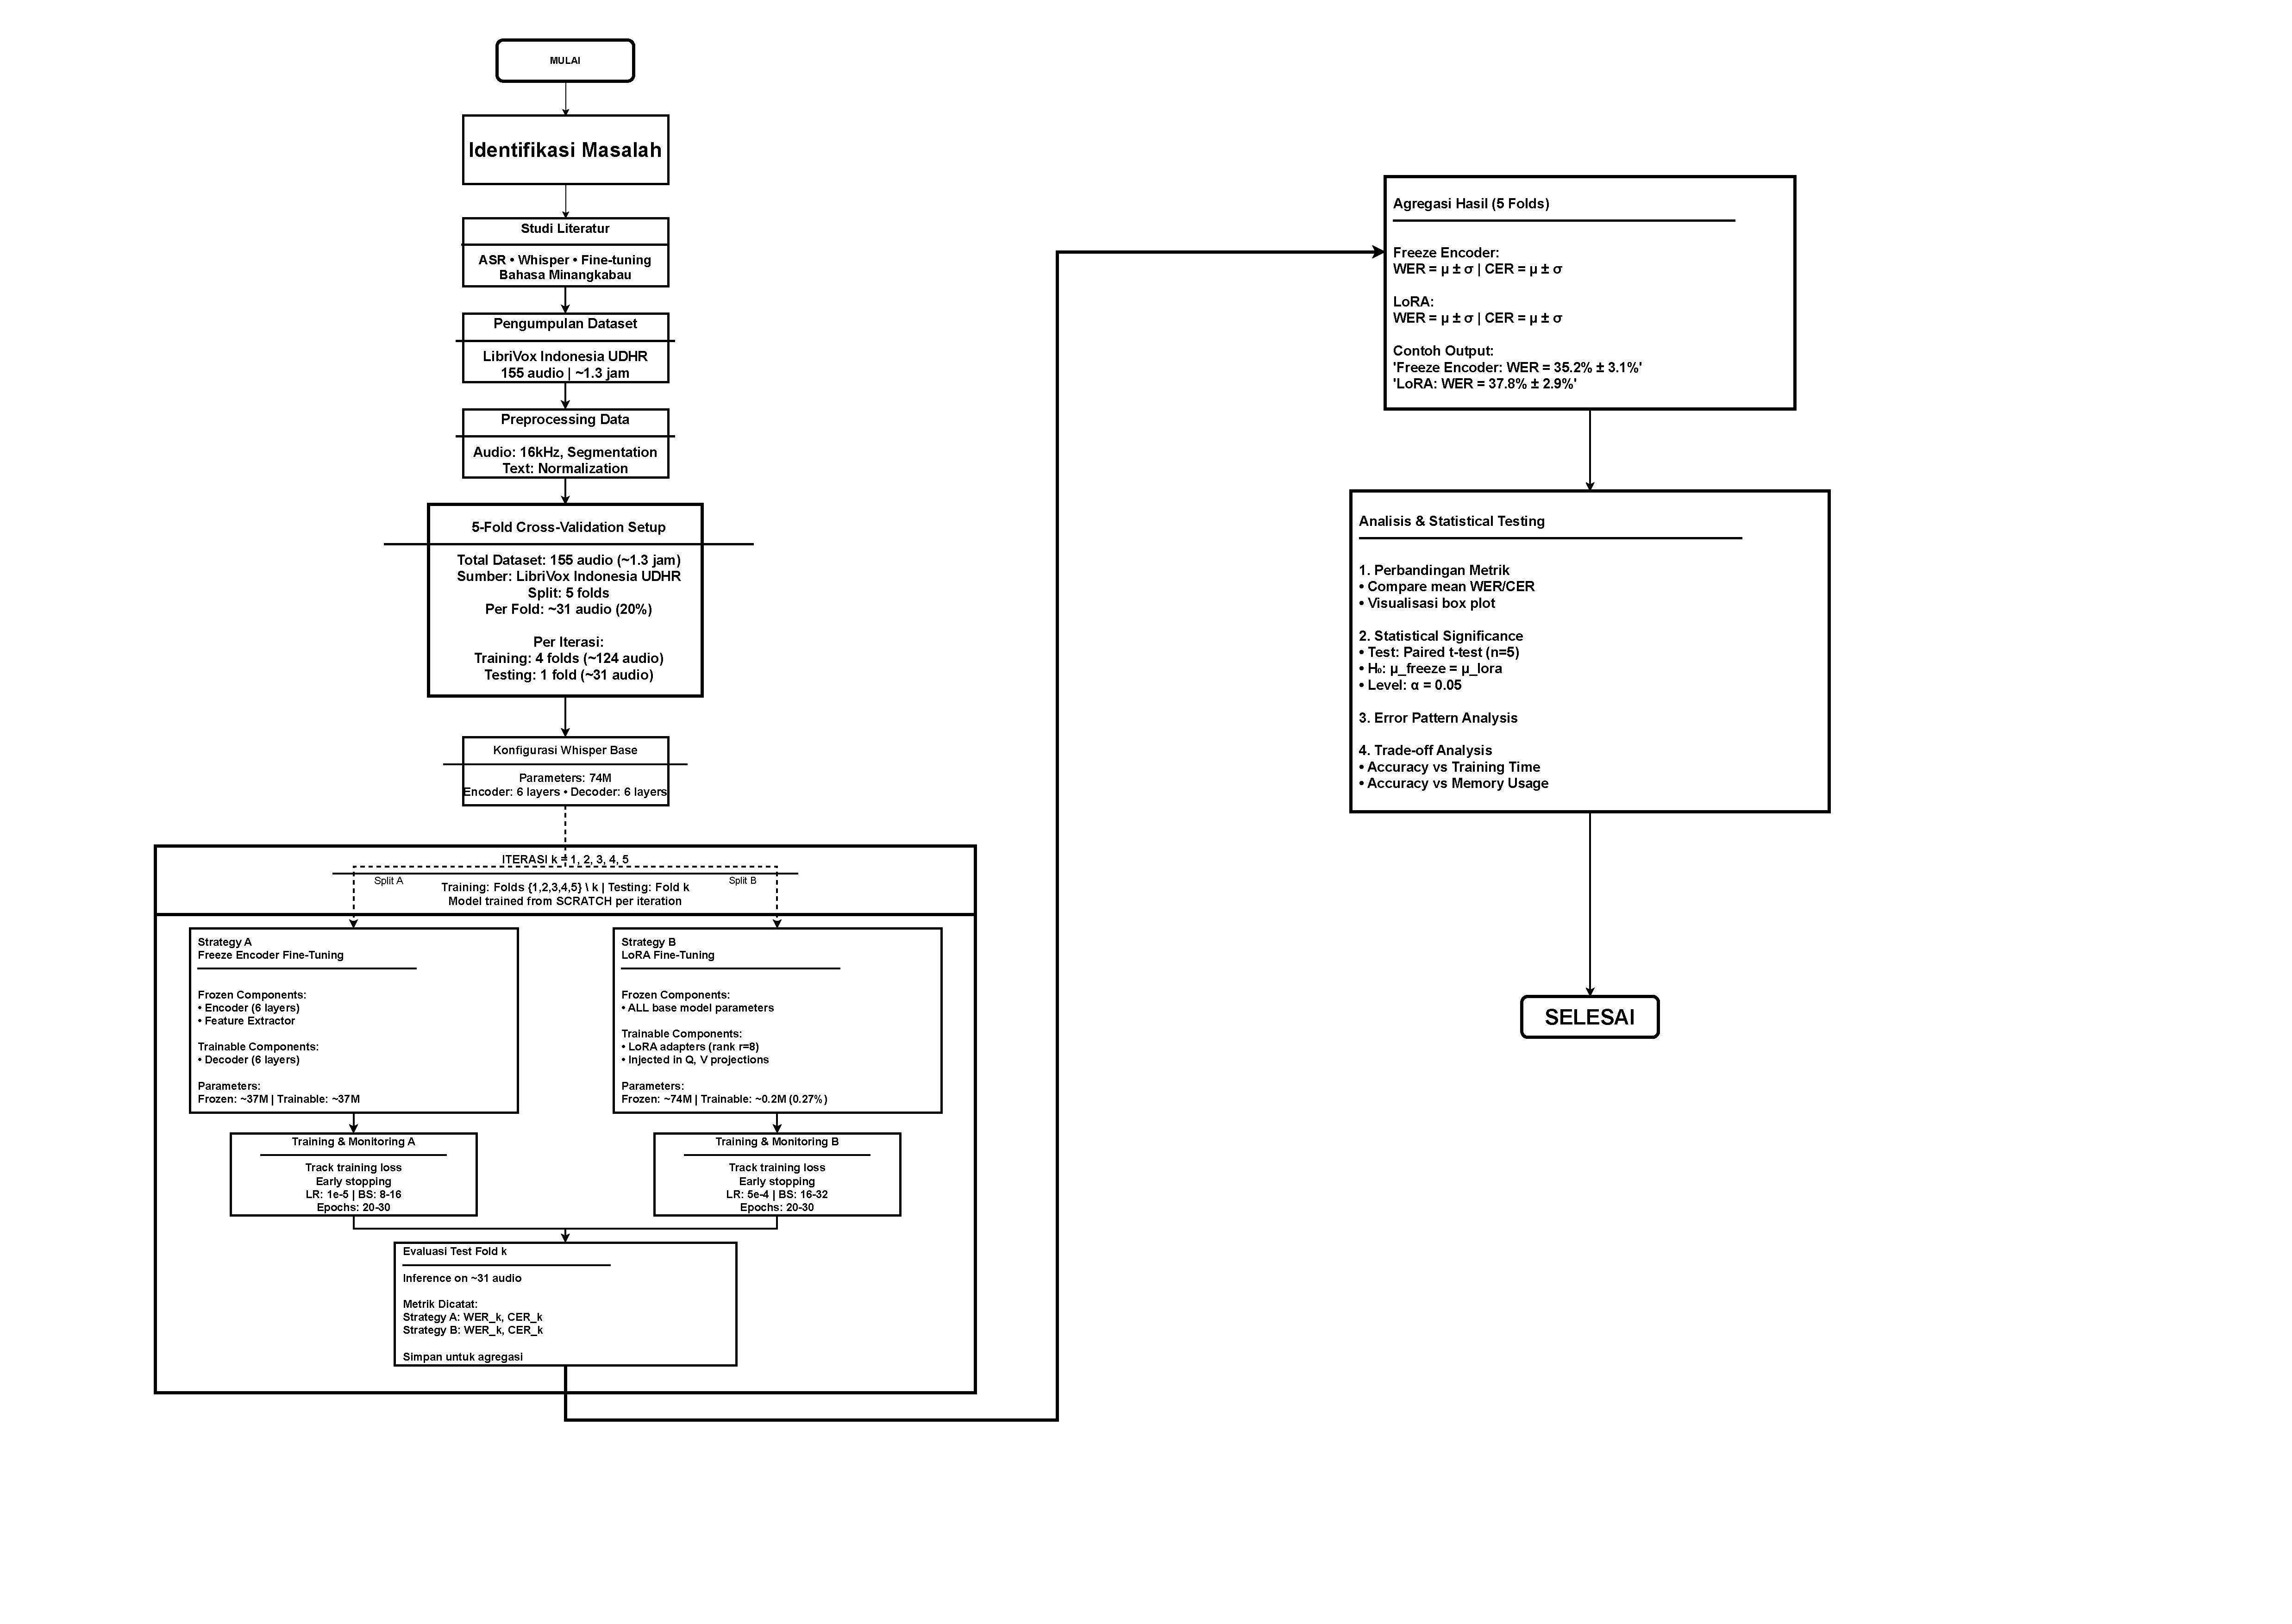
\includegraphics[width=0.55\textwidth]{../figure/Alur_Penelitian.pdf}
                \caption{Flow penelitian pada skripsi}
            \end{figure}
        \end{column}
        \begin{column}{0.44\textwidth}
            \textbf{Skema Eksekusi Eksperimen}
            \begin{itemize}
                \item 5-fold \textit{cross-validation} pada 156 audio.
                \item Setiap fold: 4 fold \textit{train}, 1 fold \textit{eval}.
                \item Augmentasi \textbf{hanya} pada data \textit{train}.
                \item \textit{Early stopping} berbasis WER evaluasi.
            \end{itemize}
        \end{column}
    \end{columns}
\end{frame}

\begin{frame}{Pipeline Preprocessing \& Augmentasi}
    \begin{columns}[T]
        \begin{column}{0.5\textwidth}
            \textbf{Audio \& Teks Preprocessing}
            \begin{itemize}
                \item Konversi MP3 $\rightarrow$ WAV, \textit{resampling} ke 16 kHz.
                \item Normalisasi amplitudo dan \textit{silence trimming}.
                \item \textit{Lowercase}, normalisasi tanda baca, pembersihan teks.
            \end{itemize}
        \end{column}
        \begin{column}{0.5\textwidth}
            \textbf{Data Augmentation (train-only)}
            \begin{itemize}
                \item \textit{Speed Perturbation}: faktor 0.85--1.15.
                \item \textit{Noise Injection}: SNR 10--30 dB.
                \item \textit{Pitch Shift}: $\pm$2 semitone.
                \item \textit{SpecAugment}: \textit{time/frequency masking}.
            \end{itemize}
        \end{column}
    \end{columns}
\end{frame}